\PassOptionsToPackage{force}{filehook}

\documentclass{beamer}
\usecolortheme{wolverine}
\setbeamertemplate{footline}[frame number]
%\useoutertheme{split}
%\useinnertheme{rounded}
\usepackage{pgf,tikz}
\usetikzlibrary{positioning}
\usepackage{amsmath}
\usepackage{amsfonts}
\usepackage{graphicx} 
\usepackage{subcaption}
\usepackage{hyperref}
\usepackage{cancel}
\usepackage{wrapfig}
\usepackage{comment}
\hypersetup{
	colorlinks=true,
	linkcolor=blue,
	filecolor=magenta,      
	urlcolor=cyan,
}
\usepackage{color}
\usepackage{mathpazo}
\usepackage{hyperref}
\usepackage{multimedia}
\usepackage{graphicx}
%\usepackage[demo]{graphicx}
\usepackage{caption}
\usepackage{subcaption}
\usepackage{textcomp}
\usepackage{graphicx} 
\usepackage{booktabs}
\usepackage{cite}
\usepackage{hyperref}
\usepackage{multicol}
\usepackage{multirow,array}
\usepackage{amsmath}
\usepackage{mathrsfs}
\usepackage{amssymb}
\usepackage[utf8]{inputenc}
\usepackage{amsthm}
\newtheorem{thm}{Teorema}
\newtheorem{lem}[thm]{Lema}
\newtheorem{axiom}[thm]{Axioma}
\newtheorem{prop}[thm]{Proposici\'on}
\newtheorem{cor}[thm]{Corolario}
\theoremstyle{definition}
\newtheorem{defn}{Definici\'on}
\DeclareGraphicsExtensions{.pdf,.jpeg,.png,.eps}
%\usetheme{CambridgeUS}
\setbeamertemplate{navigation symbols}{}
\usepackage{pgf,tikz}
\usetikzlibrary{positioning}
\usepackage[spanish, activeacute]{babel} %Definir idioma español
\usepackage[utf8]{inputenc} %Codificacion utf-8
\usepackage{multirow}
\def\mydate{\leavevmode\hbox{\twodigits\day/\twodigits\month/\the\year}}
\def\twodigits#1{\ifnum#1<10 0\fi\the#1}

\definecolor{rosee}{rgb}{0.7,0.05,0.25}


\title{Microeconom\'ia}
\subtitle{Minimizaci\'on de Costos. Corto y Largo Plazo. Funci\'on de Oferta - 1/2\\ \mydate}
\author[Minimización costos 1/2]{Lara Sánchez Peña\footnote{Basado en las notas de Marcos Ariel Lissauer}}
\institute[]{UTDT}
\medskip
\date[UTDT 2023]{}
% - Either use conference name or its abbreviation.
% - Not really informative to the audience, more for people (including
%   yourself) who are reading the slides online

%\subject{}}
% This is only inserted into the PDF information catalog. Can be left
% out. 

% If you have a file called "university-logo-filename.xxx", where xxx
% is a graphic format that can be processed by latex or pdflatex,
% resp., then you can add a logo as follows:

% \pgfdeclareimage[height=0.5cm]{university-logo}{university-logo-filename}
% \logo{\pgfuseimage{university-logo}}

% Delete this, if you do not want the table of contents to pop up at
% the beginning of each subsection:
%\AtBeginSubsection[]
%{
  %\begin{frame}<beamer>{Outline}
    %\tableofcontents[currentsection,currentsubsection]
  %\end{frame}
%}

% Let's get started
\begin{document}
\begin{frame}
  \titlepage
\end{frame}

\begin{frame}{Objetivos}
\begin{itemize}\small
    \item  ¿Por qué necesariamente una firma minimiza el costo de producción para producir una cantidad $\overline{y}$? ¿Cómo se relaciona con que una firma que maximiza beneficios necesariamente produce eficientemente?
    
    \item  En la minimización de costos, ¿qué diferencia hay entre el corto y el largo plazo?
    \item ¿Cuál es la condición para elegir óptimamente insumos $x_1, x_2$ de manera que se minimicen costos en el largo plazo? (\S 7)
    \item ¿En qué se diferencian las demandas condicionadas e incondicionadas de insumos?
    \item Función de costos y propiedades.
    \item ¿Cómo cambia el costo (m\'inimo) si aumenta en el \textbf{margen} $w_1$? \textbf{Lema de Shephard.}
    \item Gráficos de las curvas de costos y cómo se relacionan entre sí.
    \item Rendimientos a escala y función de costos, ¿cómo se relacionan?
    \item Material de repaso: Ver las slides de Eco 1 en el campus 5.2 y 5.3 + archivo de GeoGebra rendimientos.
\end{itemize}
    
\end{frame}

\begin{frame}{Introducci\'on}
\begin{itemize}\small
\item Supongamos que una firma quiere producir $\overline{y}$. Los ingresos son $p \overline{y}$ mientras que los costos podrían variar según qué combinación de insumos $(x_1,x_2)$ se use para producir $\overline{y}$. Si o si la firma produce eficientemente, $f(x_1,x_2)=\overline{y}$, sino no maximizaría beneficios. Al minimizar los costos la firma está maximizando los beneficios.
%Si una firma está maximizando sus beneficios y decide ofrecer el nivel de producción \textbf{y}, debe estar minimizando el costo de producirlo, ya que, de lo contrario, existiría una forma más barata de obtener $y$ unidades de producción, lo que significaría que la firma no estaría maximizando los beneficios.
\item Podemos dividir el problema de la firma en dos partes:
%Esta observación es útil para analizar la conducta de la firma. En efecto, el problema de la maximización del beneficio puede dividirse en dos fases:
\begin{itemize}
\item 1º, minimizar los costos al producir una cantidad $\overline{y}$. De este problema se obtiene la función de costos $C(y)$. %se averigua cómo se minimizan los costos de producir una cierta cantidad. Este es el problema de \textbf{minimización de costos}. De este problema se obtiene la \textbf{función de costos} $C(y)$ que mide lo mínimo que cuesta producir $y$ unidades.
\item 2º, \textbf{conociendo} $C(y)$, la firma elige \textbf{qué cantidad} $y$ maximiza los beneficios.
\end{itemize}

		\item Separamos el problema de la firma en dos etapas porque cualquier firma \textbf{sea competitiva o no} va a resolver el problema de minimización de costos. Cuando veamos firmas no competitivas en el mercado del bien $y$, van a poder resolver el problema de minimización de costos (vamos a asumir que en los mercado de los insumos 1 y 2 -en esta materia- sí son competitivas).
  
%  \item Es importante notar que si bien el problema de maximización no siempre tiene soluci\'on (por ej. si hay rendimientos a escala crecientes), \textbf{el problema de minimización de costos siempre la tiene}. 
		
		%\item Segundo, \textbf{mientras que el problema de maximización de beneficios es útil cuando la firma es perfectamente competitiva}. %En cambio, mientras la firma sea todav\'{i}a competitiva en el mercado de factores, el problema de minimizaci\'{o}n de costos sigue siendo v\'{a}lido bajo cualquier estructura de mercado en el mercado del bien final.
%		\item  Cuando queremos maximizar beneficios directamente, tenemos que encontrar las demandas óptimas para cada uno de los insumos para poder ver cuánto va a querer vender la firma. Si minimizamos costos primero, el problema de maximización de beneficios dependerá solamente de la cantidad $q$ que se quiere producir.
		
		%Por \'{u}ltimo, desde un punto de vista puramente anal\'{\i}tico, es generalmente m\'{a}s f\'{a}cil resolver el problema en dos etapas que hacerlo todo junto. En particular, se simplifica enormemente la condici\'{o}n de segundo orden, que con muchos factores se puede volver engorrosa.
	\end{itemize}
\end{frame}

\begin{frame}{Minimización de costos en el corto plazo}
	\begin{itemize}
		\item Supongamos una firma caracterizada por la funci\'{o}n de producci\'{o}n $f(x_{1},x_{2})$ y que $x_2=k$. Para una cantidad $\overline{y}$, sabemos que la firma producirá de manera eficiente: 
  \[f(x_1,k)=\overline{y}\]
  
  Luego, el problema que resuelve la firma es:
		\begin{equation*}
		\min_{x_{1}}w_{1}x_{1}+w_{2}k \quad s.a. \quad \overline{y}=f(x_{1},k), x_{1}\geq 0,x_{2}\geq 0
		\end{equation*}

En este caso se sabe que $x_2=k$ y la cantidad utilizada de $x_1$ se despeja de $f(x_1,k)=\overline{y}$. 

En el corto plazo, con dos insumos, hay una única manera de minimizar el costo.
		
		\end{itemize}
		\end{frame}
		

\begin{frame}{Minimización de costos en el largo plazo}
	\begin{itemize}
		\item Supongamos una firma caracterizada por la funci\'{o}n de producci\'{o}n $f(x_{1},x_{2})$. Dado que la firma quiere producir una cantidad $\overline{y} $, buscamos la ``mejor'' de hacerlo, es decir, la
combinaci\'{o}n de insumos que minimiza el costo de producci\'{o}n. Luego, el problema que resuelve la firma es:
		\begin{equation*}
		\min_{x_{1},x_{2}}w_{1}x_{1}+w_{2}x_{2} \quad s.a. \quad \overline{y} =f(x_{1},x_{2}), x_{1}\geq 0,x_{2}\geq 0
		\end{equation*}
		\item Hay dos formas de resolverlo:
		\begin{enumerate}
		    	    \item derivando y obteniendo condiciones de primer orden
	    \item analizando caso por caso (\underline{por ejemplo:} sustitutos perfectos, complementarios perfectos)
		\end{enumerate}
  \item Ejemplo del caso 1: $f(x_1,x_2)=x_1^{1/3}x_2^{1/3}$
		\end{itemize}

  
		\end{frame}
		
		\begin{frame}{Minimización de costos en el largo plazo  - Caso 1} \small
		\begin{itemize}
		
		\item Utilizamos el m\'etodo de Lagrange para resolverlo:
		\begin{equation*}
		\mathcal{L}(x_{1},x_{2},\mu)=w_{1}x_{1}+w_{2}x_{2}-\mu(f(x_{1},x_{2})-y)
		\end{equation*}
		\item ¿En qué unidades está $\mu$? ¿Qué mide?
				\item Condiciones de primer orden:
		\begin{equation*}
		w_{1}-\mu^{c}\frac{\partial f(x^{c}_{1},x^{c}_{2})}{\partial x_{1}}=0
		\end{equation*}
		\begin{equation*}
		w_{2}-\mu^{c}\frac{\partial f(x^{c}_{1},x^{c}_{2})}{\partial x_{2}}=0
		\end{equation*}
		\begin{equation*}
		y-f(x^{c}_{1},x^{c}_{2})=0
		\end{equation*}
	

		\item La soluci\'on a este problema ser\'an  $x^{c}_{1}(w_{1},w_{2},\overline{y}), x^{c}_{2}(w_{1},w_{2},\overline{y})$ y las llamaremos \textbf{demandas condicionadas}. 
		\item Notar que reordenando las CPO obtenemos la relaci\'on:
		\begin{equation*}
			TMST(x_{1}^c,x_{2}^c)=\frac{PMg_{1}(x^{c}_{1},x^{c}_{2})}{	PMg_{2}(x^{c}_{1},x^{c}_{2})}=\frac{w_{1}}{w_{2}}
		\end{equation*}
	
	\end{itemize}
\end{frame}	


	
	\begin{frame}{Minimización de costos - Caso 2}
	Veamos como resolver dos ejemplos:
\begin{center}
\begin{tabular}{c|c}
\hline
   $f(x_1,x_2)=2x_1+x_2$  &  $f(x_1,x_2)=\min \{2x_1,x_2\}$  \\
   \hline
     & \\
 \color{gray} ¿Qué pasa si $\frac{w_1}{w_2}<2$?     & \\
  \color{gray}Solamente se usa $x_1$.   & \color{gray} ¿Por qué la firma elige\\ 
     & \color{gray} $2x_1=x_2$ para minimizar costos?\\
     & \\
 \color{gray} ¿Qué pasa si $\frac{w_1}{w_2}>2$?      & \\
 \color{gray}Solamente se usa $x_2$.     & \\
     & \\
    & \\
   \color{gray} ¿Qué pasa si $\frac{w_1}{w_2}=2$?    & \\
  \color{gray} La firma está indiferente entre   & \\
  \color{gray} usar insumo $1$ o $2$.    & \\
     & \\
\end{tabular}
   \end{center}
    
\end{frame}	
\begin{frame}{Minimización de costos - en general}
	\begin{itemize}
 \item \small{Notar que, \textbf{si tenemos una solución de esquina en la que no se utiliza uno de los factores, no necesariamente se satisface que $TMST=\dfrac{w_1}{w_2}$ y sin embargo es óptimo.} Por ejemplo, si $f(x_1,x_2)=2x_1+x_2$. ¿Qué ocurre en ese caso?}
\item Supongamos que $\frac{w_{1}}{w_{2}}=3$, entonces:
\begin{align}
TMST(x_{1},x_{2})=2<\frac{w_{1}}{w_{2}}=3 \label{eq}
\end{align}
\item \small{Para producir óptimamente no utilizamos, en este caso, el insumo 1 porque si bien el insumo 1 es el doble de productivo que el insumo 2 cuesta el triple.}
%Podr\'iamos disminuir cu\'anto usamos del insumo 1 en \textbf{dos} unidades y aumentar el insumo 2 en \textbf{una} unidad y mantendr\'{\i}amos constante el nivel de producto (porque la $TMST=2$) y eso implicaría disminuir los costos, pues el insumo 1 sale el triple que el 2.

\item \small{Del mismo modo, \textbf{si la función
de producción no es suave} (su TMST no varía de manera continua), no necesariamente se cumple que $TMST(x_1^C,x_2^C)=\dfrac{w_1}{w_2}$ y sin embargo es óptimo. Por ejemplo, si $f(x_1,x_2)=\min\lbrace 2x_1,x_2\rbrace$. Para esta tecnología Leontief $TMST(x_1,x_2)=\begin{cases} 0 &\text{ si } 2x_1 \geq x_2\\  +\infty &\text{ si } 2x_1 <x_2\end{cases}$} %¿Qué ocurre en ese caso?} %Estas situaciones son similares a las que encontramos en el caso del consumidor.

\end{itemize}
\end{frame}	

\begin{frame}{Demandas no condicionadas $x^*$ vs condicionadas $x^C$}
\begin{itemize}
\item Es importante notar la diferencia entre: 
\begin{enumerate}
    \item las demandas \textbf{condicionadas} $x_i^C(w_1,w_2,y)$ para $i=1,2$ que encontramos en el problema de \textbf{minimización de costos} y 
    \item las demandas \textbf{no condicionadas} $x_i^*(w_1,w_2,p)$ para $i=1,2$ que encontramos en el problema de \textbf{maximización de beneficios}.
\end{enumerate} 
\item Si minimizamos costos, encontramos las demandas \textbf{condicionadas} a una cantidad específica de producto que se quiere producir $y$. Es decir, \textbf{tomando como dado el nivel de producto} $y$ que se quiere alcanzar. 
\item Las demandas \textbf{incondicionadas} son las
que nos permiten obtener el mayor beneficio \textbf{tomando como dados los precios} (de los insumos y del bien final). A partir de las demandas incondicionadas determinamos la oferta de producto $y(p,w_1,w_2)=S(p)$.
\end{itemize}
\end{frame}	

\begin{frame}{Minimización de costos - solución gráfica}
\begin{itemize}
\item Veamos gr\'{a}ficamente el problema de minimización de costos. 

\begin{enumerate}
    \item \small{Graficamos la \textbf{isocuanta} sobre la cual deseamos producir. Es decir combinaciones} $\left( x_{1},x_{2}\right)$ \small{tal que} $\overline{y}=f(x_{1},x_{2})$.
    \item Graficamos las \textbf{rectas isocosto}, \small{las combinaciones de} $\left( x_{1},x_{2}\right)$ \small{tal que obtenemos un costo constante igual a} $C$. Son rectas porque $w_1$ y $w_2$ están dados.
\end{enumerate} 
\[C =w_{1}x_{1}+w_{2}x_{2} \Leftrightarrow x_{2} =\frac{C}{w_{2}}-\frac{w_{1}}{w_{2}}x_1\]\par
	\begin{center}
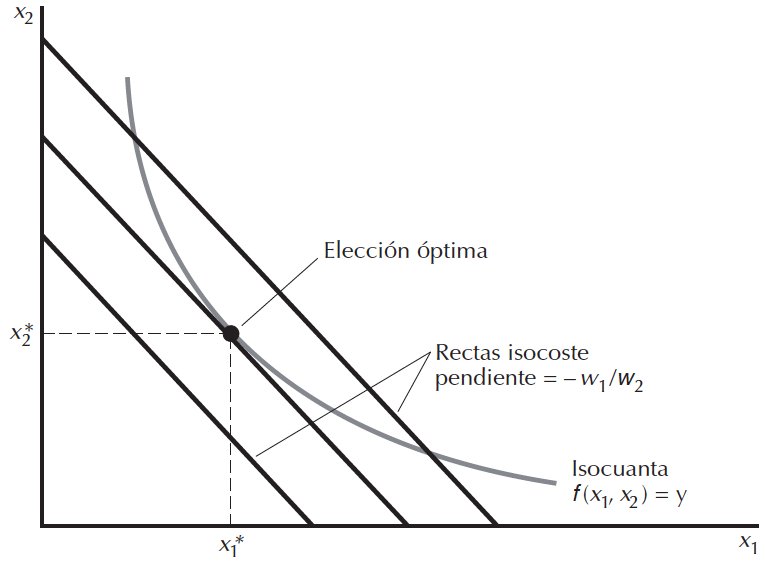
\includegraphics[width=2in]{figures4/isocost.png}
\end{center}
\end{itemize}
\end{frame}		

\begin{frame}{Funci\'on de costo (m\'inimo)}\small
\begin{itemize}
\item Una vez obtenidas las demandas condicionadas de insumos, las reemplazamos
en la funci\'{o}n de costo y obtener  la \textit{funci\'on de costo (m\'{\i}nimo):}
\end{itemize}
\begin{equation*}
C(w_{1},w_{2},y)=w_{1}x^{c}_{1}(w_{1},w_{2},y)+w_{2}x^{c}_{2}(w_{1},w_{2},y)
\end{equation*}
\begin{itemize}
\item Por ejemplo, si la funci\'on es Leontief, $f(x_1,x_2)=\min\big\{2x_1,x_2\big\}$. Luego, $2x_1=x_2=y$ por lo que la funci\'on costo m\'inimo ser\'a $C(w_{1},w_{2},y)=w_1\frac{y}{2}+w_2y=\left(\frac{w_1}{2}+w_2\right)y$.
\item Si $f(x_1,x_2)=2x_1+x_2$, dado que los factores 1 y 2 son sustitutos perfectos en la producción, la firma usará $\frac{1}{2}$ unidad del insumo 1 o $1$ unidad del insumo $2$ para producir una unidad de bien final. Qué insumo(s) se use(n) dependerá de comparar $\frac{w_1}{2}$ y $w_2$. El costo mínimo de $y$ unidades de producción será el menor de $\frac{w_1}{2}y$ o $w_2y$. Es decir, $C(w_{1},w_{2},y)= \min\left\{\frac{w_1}{2},w_2\right\}y$.
\item ¿Por qué sucede esto? ¿Cómo sería la función de costo mínimo si la tecnología es Cobb-Douglas, por ejemplo, $f(x_1,x_2)=x_1^{1/3}x_2^{1/3}$?
\end{itemize}
\end{frame}

\begin{frame}{Est\'atica comparativa en el largo plazo}
	\begin{itemize}
	\item \textbf{Queremos analizar c\'{o}mo cambian las variables endógenas que maximizan beneficios} $(x_1^c,x_2^c,C(\cdot))$ \textbf{si cambia alg\'{u}n factor que consideramos ex\'{o}geno} $(w_1,w_2, y)$. 
	
\begin{center}
\begin{tabular}{|c|c|c|c|}
\hline
&$x_1^C$ & $x_2^C$&  $C(\cdot)$\\[6pt] 
\hline 
$\frac{\partial}{\partial w_1}$ & \color{cyan} $\leq 0$ & \color{rosee} $\geq 0 $&\color{rosee}$\geq 0$\\[6pt]
\hline
$\frac{\partial}{\partial w_2}$ &\color{rosee} $\geq 0$& \color{cyan} $\leq 0$&\color{rosee} $\geq 0$\\[6pt]
\hline
$\frac{\partial}{\partial y}$ &\color{rosee}$\geq 0$&\color{rosee}$\geq 0$&\color{rosee}$\geq 0$\\[6pt]
\hline
\end{tabular}
\end{center}

  \end{itemize}

  
\end{frame}	


\begin{frame}{Propiedades de las $x^C$ y de la función de costos }

La funci\'on de costo y demandas condicionadas tienen algunas propiedades de
inter\'es:
\begin{itemize}
	\item $\frac{\partial x^{c}_{i}}{\partial w_{i}}\leq 0$\footnote{ \, Si aumenta el precio $w_i$ se demanda menos insumo $x_i^c$ o lo mismo. Se podría demandar lo mismo si, por ejemplo $x_1^c=0$. \textbf{Los insumos $x_i^c$ son bienes ordinarios}.}
	\item $x^{c}_{i}(tw_{1},tw_{2},y)=x^{c}_{i}(w_{1},w_{2},y)$\footnote{\, $x_i^c$ es HOD 0 en $(w_1,w_2)$. Si aumenta los dos precios $w_1$ y $w_2$ en la misma proporción, como ninguno de los insumos es relativamente más barato, para producir $y$ demando lo mismo de cada insumo en ambos casos.} 
	\item $C(tw_{1},tw_{2},y)=tC(w_{1},w_{2},y)$\footnote{ \, Ver nota al pie \textit{b}, el costo se multiplica por $t$.}
	\item \textbf{Lema de Shephard}: $\frac{\partial C}{\partial w_{i}}=x^{c}_{i}(w_{1},w_{2},y)$\footnote{    \, Partiendo de $(x_1^c,x_2^c)$ que minimizan costos, si aumenta apenas $w_i$ entonces la función de costos aumenta en $x_i^c$. Los demás efectos son pequeños. }
	\end{itemize}
	
\end{frame}

\begin{frame}{Rendimientos a escala}

\begin{prop}
A partir de la funci\'{o}n de costos, podemos identificar r\'{a}pidamente el
tipo de rendimientos a escala de la tecnolog\'{\i}a de producci\'{o}n. Los rendimientos a escala y la funci\'{o}n de costos medios se relacionan:\footnote{\,Recordar que si $f(0,0)=0$ y además:
\begin{enumerate}
\item $f$ es convexa, entonces $f$ exhibe IRS.
\item $f$ es lineal, entonces $f$ exhibe CRS.
\item $f$ es cóncava, entonces $f$ exhibe DRS.
\end{enumerate}}
\begin{enumerate}
\item $f$ tiene \textbf{rendimientos crecientes a escala}  $\Leftrightarrow \frac{\partial
CMe}{\partial y}<0\Leftrightarrow CMe(y)>CMg(y) \Leftrightarrow C(y)$ es cóncava.
\item $f$ tiene \textbf{rendimientos constantes a escala} $\Leftrightarrow \frac{\partial
CMe}{\partial y}=0\Leftrightarrow CMe(y)=CMg(y)$. Si valen $\forall y \Leftrightarrow C(y)=c\cdot y$ es lineal.
\item $f$ tiene \textbf{rendimientos decrecientes a escala}  $\Leftrightarrow \frac{\partial
CMe}{\partial y}>0\Leftrightarrow CMe(y)<CMg(y) \Leftrightarrow C(y)$ es convexa.
\end{enumerate}
\end{prop}
\end{frame}

\begin{frame}{Rendimientos a escala - intuición}
\begin{itemize}
\item Veamos la intuición para el caso (3). Supongamos que
la tecnología de producci\'{o}n tiene \textbf{rendimientos decrecientes a escala}. Esto
implica, que, por ejemplo, para duplicar la producci\'{o}n se requiere
más del doble que los insumos.\footnote{ \, Esto es análogo a decir que si se duplican los insumos no alcanza para duplicar la cantidad producida.} 

\item Eso implica que, si se duplica la
producci\'{o}n, el costo es más que el doble. Por lo tanto, aumenta el costo medio $(\frac{\partial CMe}{\partial y}>0)$. 
\item Entonces, si el costo medio es creciente, debe suceder que $CMe(y)<CMg(y)$. 
\item Eso implica que $CT$ es convexo. La idea es que como el $CMe$ es creciente, el $CMg$ tiene que \textbf{aumentar cada vez más rápido} (o sea $C''(y)>0$) de manera que aumente el valor promedio.
\item Practiquen escribir qué sucedería en los demás casos.
\end{itemize}
\end{frame}

%\begin{frame}{Dos propiedades útiles de la función de costos}
 %   \begin{prop}
  %  Si $f(x_1,x_2)$ tiene rendimientos constantes a escala, entonces la función de costos es $C(w_{1},w_{2},y) = c(w_{1},w_{2}) y$.
 %   \end{prop}
    
%\begin{prop}
%Si $f(x_1,x_2)$ es cóncava y $f(0,0)=0$ (si $f$ tiene DRS), entonces $C(y)$ es convexa en $y$.
%\end{prop}
%\end{frame}

\begin{frame}{\small Curvas de costos marginal y medios para una tecnología más genérica}
    Imaginemos una tecnología que no cae en las categorías DRS, CRS, IRS. ¿Cómo se verían gráficamente las curvas de costo marginaly medio?
    \begin{itemize}
        \item Supongamos que la firma tiene para cantidades pequeñas ``rendimientos crecientes a escala''.
        \item Supongamos que la firma tiene para una cantidad $\overline{y}$ (la escala eficiente - donde se minimiza el costo medio) ``rendimientos constantes a escala''.
        \item Supongamos que la firma tiene para cantidades mayores ``rendimientos decrecientes a escala''.
    \end{itemize}

    Vamos a graficar $CMg(y)$, $CMe(y)$ y $CMeV(y)$. Si no hay costos fijos $CMe(y)=CMeV(y)$.
\end{frame}

%\begin{frame}{Curva de costos}
%\begin{itemize}
%\item \textbf{Veamos gráficamente propiedades de la función de costos.}
%\item Recordemos que la curva de costos $C\left( w_{1},w_{2},y\right) $ establece el costo m\'inimo de producir una
%cantidad de bien final $y$ tomando como dados los precios de los insumos $\left( \textbf{w}\right) $. 
%\item Como vimos en la secci\'{o}n anterior, en el corto plazo, pueden existir costos que se pagan independientemente del nivel de producci\'{o}n de bien final $y$. Estos costos son \textbf{fijos}. En contraste, los \textbf{costos variables} son el resultado de pagar por los insumos para la producci\'{o}n. Luego,
%\begin{equation*}
%C\left( w,y\right) =c_{v}\left( w,y\right)+F
%\end{equation*}
%donde $F$ representa los costos fijos y $c_{v}\left(
%w,y\right) $ los variables. En el ejemplo de corto plazo, %$c_{v}\left( w,y\right) =w_{1}x_{1}$ y $F=w_{2}k$.
%\end{itemize}
%\end{frame}

\begin{frame}{Costo medio para una tecnología más genérica}%\small

%Consideremos una tecnología que, para cantidades producidas de bien final 
%\begin{itemize}
%    \item ``bajas'' indicaría que como si hubiera ``rendimientos crecientes a escala''
%    \item ``intermedia'' la firma alcanza la \textbf{escala de producción} (donde el costo medio se minimiza) - a ese tramo se lo asocia con ``rendimientos constantes a escala''
%    \item ``altas'' indicaría como si hubiera ``rendimientos crecientes a escala''
%\end{itemize}


A partir de la funci\'{o}n de costo m\'inimo (total) podemos definir otras
curvas de costos que ser\'{a}n de nuestro inter\'{e}s:
\begin{itemize}
\item \textbf{Costo medio:} mide el costo por unidad de bien final, es decir, el costo
promedio por unidad. El costo medio tiene dos partes:
\begin{enumerate}
    \item costo medio variable $CMeV(y)$ y \vspace{3pt}
    \item costo medio fijo $CMeF(y)=\frac{F}{y}$:
\end{enumerate}

\begin{align*}
CMe\left( y\right) =\frac{C\left( y\right) }{y}=\frac{c_{v}\left( y\right) }{%
y}+\frac{F}{y}=CMeV\left( y\right) +CMeF\left( y\right)
\end{align*}
\end{itemize}
\end{frame}

\begin{frame}{\small Costo medio variable, fijo y total para una tecnología más genérica}
\begin{itemize}
\item  $CMeF\left( y\right)\xrightarrow{y\to +\infty} 0$ y $CMeF\left( y\right)\xrightarrow{y\to 0} +\infty$. \textbf{(Ver gráfico A}). 
\item Respecto a $CMeV\left(y\right) $, uno esperaría que inicialmente el $CMeV(y)$ fuera constante y/o luego creciente. \textbf{(Ver gráfico B}). 

\item El costo medio (total) va a ser \textbf{(Ver gráfico C}) que es la suma horizontal de los gráficos \textbf{A} y \textbf{B}.
%\begin{itemize}
%    \item creciente si la tecnología $f(x_1,x_2)$ exhibe $DRS$.
%    \item decreciente si la tecnología $f(x_1,x_2)$ exhibe $IRS$.
%    \item constante si la tecnología $f(x_1,x_2)$ exhibe $CRS$.
%\end{itemize}
%el costo medio variable de producir una unidad es exactamente el costo variable total. Ahora aumentemos el nivel de producción a 2 unidades. Cabe esperar que, quiz\'as, los costos variables se dupliquen y que, por tanto, los costos variables medios permanezcan constantes. 
%\item Si podemos organizar la producción de modo que al aumentar la escala de producción vayamos ganando en eficiencia, los costos variables medios pueden llegar a disminuir. 
%\item Sin embargo, a la larga, hay que contar con que aumenten. ¿Por qué? Porque si hay factores fijos, éstos acaban limitando la capacidad de expansión del proceso productivo.
\end{itemize}

	\begin{center}
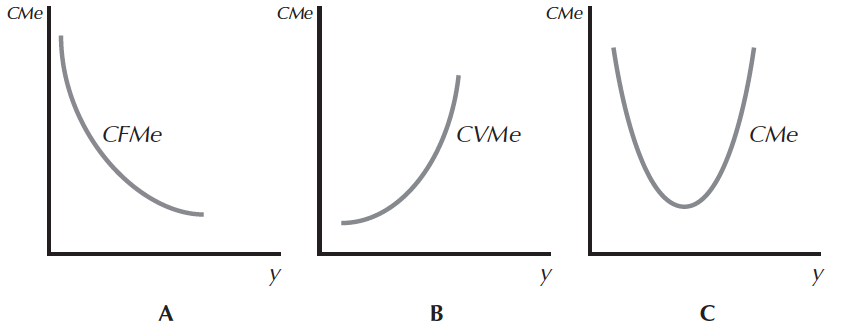
\includegraphics[width=4in]{figures4/costos.png}
\end{center}
\end{frame}

\begin{frame}{\small Relación entre \textit{CMg}, \textit{CMe} y \textit{CMeV} para una tecnología más genérica}\small
\begin{itemize}
%\item \textbf{Costo marginal:} el costo marginal mide cuánto aumenta el costo total cuando aumenta marginalmente la cantidad que se quiere producir $y$. %establece la tasa de cambio del costo total ante un cambio en el producto final deseado:
%\begin{equation*}
%CMg(y):=C'(y)=\frac{\partial C\left( y\right) }{\partial y}=\frac{\partial c_v\left(y\right) }{\partial y}
%\end{equation*}
\item \ Como los costos variables de producir cero unidades de bien final son
cero por definici\'{o}n, al incrementar marginalmente la producci\'{o}n de cero unidades a $y$,
\begin{equation*}
\lim_{y \rightarrow 0}CMg\left( y \right)
=\lim_{y
\rightarrow 0}CMeV\left( y \right)
\end{equation*}

%\begin{equation*}
%\lim_{y \rightarrow 0}CMg\left( y \right)
%=\lim_{y \rightarrow 0}\frac{c_{v}\left( y \right)
%-c_{v}\left( 0\right)}{y }=\lim_{y \rightarrow 0}%
%\frac{c_{v}\left( y \right) }{y }=\lim_{y
%\rightarrow 0}CMeV\left( y \right)
%\end{equation*}
\item \textbf{Propiedad 1:} \textit{CMg(y)} y \textit{CMeV(y)} tienen la misma ordenada al origen. %Vamos a ver más propiedades cuando veamos \textbf{rendimientos a escala}. %Es decir, cuando nos acercamos a cero, el costo medio variable se ``pega'' al costo marginal.

    \item \textbf{Propiedad 2: }la curva \textit{CMg(y)} pasa por los valores mínimos de las curvas de \textit{CMe(y)} y \textit{CMeV(y)}.\footnote{\textbf{Demostración matemática}: para encontrar el costo medio mínimo hay que derivar $CMe(y)=\frac{C(y)}{y}$. Tenemos que $CMe'(q)=\frac{C'(y)y-C(y)}{y^2}$. Para encontrar donde se minimiza $CMe(y)$, tiene que ocurrir que $\frac{C'(y)q-C(y)}{y^2}=0$, es decir, $y$ cumple que $CMe(y)=C'(y)$. Para ver el resultado con costo medio, hay que cambiar $C(y)$ por $C_v(y)$. $\qed$}
    
    \vspace{8pt}
   % La curva de costo marginal pasa por el punto mínimo tanto de la curva de costo variable medio como de la curva de costo medi

\end{itemize}
\end{frame}

\begin{frame}{Intuición de la propiedad 2}\small
\begin{itemize}
       
    
   \item Si el $CMe(y)$ es decreciente es porque al aumentar la cantidad producida $y$, (cuando se producen pocas unidades de $y$) las últimas unidades que se van produciendo tienen un $CMg(y)$ que es decreciente.
   
  \item Luego, cuando ya se produce cierta cantidad y se sigue aumentando el nivel de producción ocurre que, incluso si $CMg(y)$ va aumentando, el $CMe(y)$ es decreciente.
   
   \vspace{8pt}
   
   \item Para algún valor de $y$ las curvas de $CMe(y)$ y $CMg(y)$ se cruzan. Eso ocurre cuando el $CMe(\overline{y})$ es igual al costo de la última unidad $CMg(\overline{y})$. En ese caso $\overline{y}$ se conoce como la \textbf{escala de producción}. 
   
   \item Si el $CMg$ sigue aumentando, necesariamente $CMe$ tiene que aumentar.
   
   \vspace{8pt}
   
  \item Eso quiere decir que $CMe$ es decreciente hasta el valor de $y$ donde $CMe(y)=CMg(y)$ y luego $CMe(y)$ es creciente. Por lo tanto si $y$ cumple que $CMe(y)=CMg(y)$ ese valor es el mínimo de la curva $CMe(y)$.
   \end{itemize}
\end{frame}

%\begin{frame}{Relaci\'on entre \textit{CMg} y \textit{CMeV}}
%\begin{itemize}
%\item \textbf{Supongamos que estamos produciendo en un punto en el cual los costos medios variables son decrecientes.} Para que los \'ultimos decrezcan, debe
%suceder que cada unidad extra que se agrega sea menor que el promedio del costo variable, pues de otra manera, el promedio aumentar\'{a}. Formalmente,
%\begin{equation*}
%\frac{\partial CMeV\left( y\right) }{\partial y}=\frac{\partial }{\partial y}%
%\left[ \frac{c_{v}\left( y\right) }{y}\right] =\frac{c_{v}^{\prime }\left(y\right) y-c_{v}\left( y\right) }{y^{2}}
%\end{equation*}
%\item Por lo tanto, será decreciente cuando:
%\begin{equation*}
%c_{v}^{\prime }\left( y\right) =CMg\left( y\right) <\frac{c_{v}\left(
%y\right) }{y}=CMe(y)
%\end{equation*}
%\item Es decir, cuando el costo marginal se encuentre por debajo del medio variable. El $CMeV(y)$ será creciente si $CMg(y)>CMe(y)$. El mismo argumento vale para los costos medios totales.
%\end{itemize}
%\end{frame}

\begin{frame}{Curvas de costos para una tecnología más genérica}
	\begin{center}
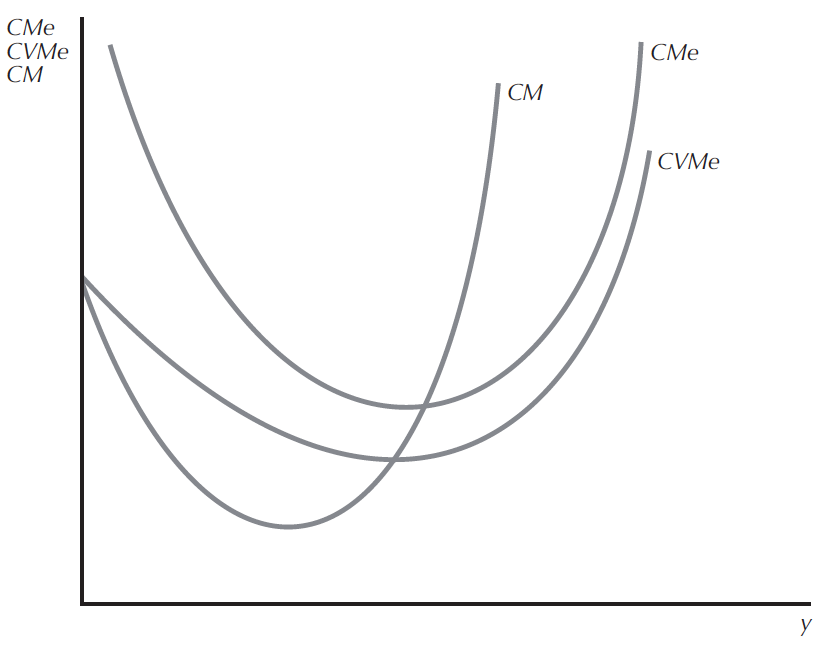
\includegraphics[width=3.8in]{figures4/costostodos.png}
\end{center}
\end{frame}





\begin{frame}{Curvas de costos - obtener \textit{CT} a partir de \textit{CMg}}\small
\begin{itemize}
\item Como $CMg\left( y\right) =\frac{\partial C\left( y\right) }{\partial y}=\frac{\partial c_{v}\left( y\right) }{\partial y}$, sucede que:
\begin{equation*}
c_{v}\left( y\right) =\int\limits_{0}^{y}CMg(v)dv
\end{equation*}
pues sabemos que $c_{v}\left( 0\right) =0$. El \'{a}rea bajo la curva $CMg$ entre $0$ e $y$, es exactamente el costo variable de
producir la cantidad $y.$
\item Como $C\left( 0\right) =F$, los costos
totales:
\begin{equation*}
C(y)=F+\int\limits_{0}^{y}CMg(v)dv
\end{equation*}
\end{itemize}
	\begin{center}
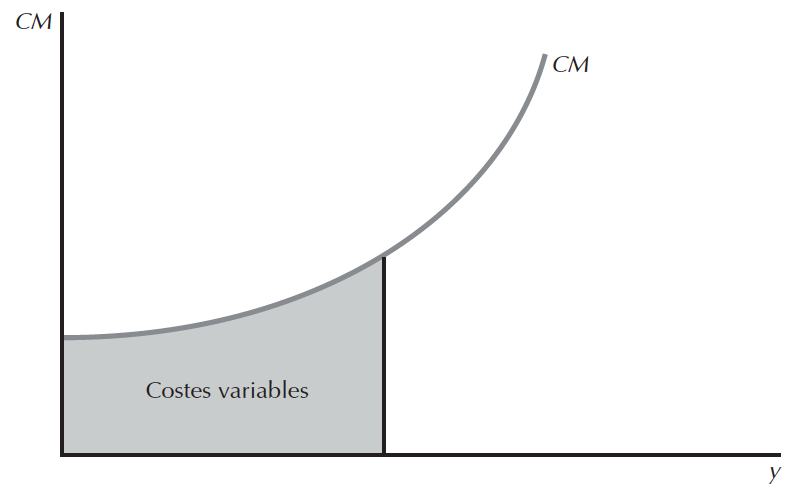
\includegraphics[width=1.8in]{figures4/CV.png}
\end{center}
\end{frame}


%\begin{frame}{Curvas de costos}
%Resumiendo:
%\begin{itemize}
%\item La \textbf{curva de costo variable medio} puede tener pendiente negativa al principio, aunque no necesariamente. Sin embargo, a la larga (NO QUEDA CLARO, además esto se ve con rendimientos más fácil) crece si hay algún factor fijo que limita la producción.
%\item La curva de costo medio puede descender al principio debido a los costos fijos medios decrecientes, pero después aumenta debido a los costos variables medios crecientes.
%\item El costo marginal y el costo variable medio de la primera unidad de producción son iguales.
%\item La curva de costo marginal pasa por el punto mínimo tanto de la curva de costo variable medio como de la curva de costo medio.
%\end{itemize}

%\end{frame}

%%%%%%%%%%%%%%%%%%%%%%%%%%%%%%%%%%%%%%%%%%%%%%%%%%%%%%%%%%%%%%%%%%%%%%%%%%%%%%%%%%%%%%%%%%%%%%%%%%%%%%%%%%%%%%%%%%%%%%%%%%%%%%%%%%%%%%%%%%%%%%%%%%%%%%%%%%%%%%%%%%%%%%%%%%%%%%%%%%%%%%%%%%%%%%%%%%%%%%%%%%%%%%%%%%


%\begin{frame}{Propiedades}
%MEJORAR ESTA SLIDE Y LA 29, ver si tengo que borrar lo ultimo que puse en la 29 (las borro y resumo todo en la 29)
%\begin{prop}
%Suponiendo que $f(0,0)=0$, (hay que agregar esto?)
%\begin{itemize}
%\item Si $f$ tiene rendimientos constantes a escala, entonces la funci\'{o}n de costos es $C(w_{1},w_{2},y)=C(w_{1},w_{2})y.$
%\item Si $f$ es c\'{o}ncava, entonces $C(y)$ es convexa en $y$.
%\item Si $f$ es convexa, entonces $C(y)$ es c\'{o}ncava en $y$.
%\end{itemize}
%\end{prop}
%\end{frame}

%\begin{frame}{Propiedades}
%\begin{itemize}
%\item Si la tecnolog\'{\i}a de producci\'{o}n exhibe CRS, la función $C(y)$ es lineal en la cantidad de bien final producido $y$. Si aumenta la cantidad de bien final producido, entonces el costo total aumentará en la misma proporción. O sea, si producimos $ty$ el costo total será $C(ty)=tC(y)$.
%\item Si la tecnolog\'{\i}a de producci\'{o}n exhibe DRS Supongamos que $f$ es c\'oncava y que se utiliza un  \'{u}nico insumo para la producci\'{o}n. Imaginemos pasar de 0 unidades producidas a 1 unidad requiere de 3 unidades del insumo, produciendo un costo total de $C=3w$. Como $f$ es c\'oncava, pasar de 1 unidades de producto final a 2 requerir\'{a} de m\'{a}s que 3 unidades de insumos extras. Por lo tanto, el costo total, ser\'{a} mayor al doble del anterior. Es decir, el costo total ser\'{a} creciente en $y$ a tasa creciente, es decir, convexo.
%\end{itemize}
%\end{frame}

\begin{frame}[noframenumbering]{Ejemplo: Cobb-Douglas (*)}

\textbf{Ejercicio}: Minimice el costo en el largo plazo para $f(x_1,x_2)=x^{\alpha}_{1}x^{\beta}_{2}$. Encuentre $x_1^C, x_2^C$ y $C(y)$.

\color{gray}
\textbf{Solución:}
		\begin{equation*}
		\min_{x_{1},x_{2}}w_{1}x_{1}+w_{2}x_{2} \quad s.a. \quad y=x^{\alpha}_{1}x^{\beta}_{2}, x_{1}\geq 0,x_{2}\geq 0
		\end{equation*}
		\begin{equation*}
		\mathcal{L}(x_{1},x_{2},\mu)=w_{1}x_{1}+w_{2}x_{2}-\mu(x^{\alpha}_{1}x^{\beta}_{2}-y)
		\end{equation*}
CPO:
\begin{equation*}
[x_{1}]: w_{1}=\mu\alpha x^{\alpha-1}_{1}x^{\beta}_{2}=\mu\alpha\frac{y}{x_{1}}
\end{equation*}		
\begin{equation*}
[x_{2}]: w_{2}=\mu\beta x^{\beta-1}_{2}x^{\alpha}_{1}=\mu\beta\frac{y}{x_{2}}
\end{equation*}		
\begin{equation*}
[\mu]: y=x^{\alpha}_{1}x^{\beta}_{2}
\end{equation*}
\end{frame}

\begin{frame}[noframenumbering]{Ejemplo: Cobb-Douglas (*)}
\color{gray}
Combinando las primeras dos condiciones:
\begin{equation*}
\frac{\alpha x_{2}}{\beta x_{1}}=\frac{w_{1}}{2_{2}}\Longleftrightarrow x_{2}=x_{1}\frac{\beta}{\alpha}\frac{w_{1}}{w_{2}}
\end{equation*}
Reemplazando en la restricci\'on:
\begin{equation*}
x^{\alpha}_{1}\left(x_{1}\frac{\beta}{\alpha}\frac{w_{1}}{w_{2}}\right)^{\beta}=y
\end{equation*}
Despejando $x_{1}$:
\begin{equation*}
x^{c}_{1}(w_{1},w_{2},y)=\left(\frac{\alpha w_{2}}{\beta w_{1}}\right)^{\frac{\beta}{\alpha+\beta}}y^{\frac{1}{\alpha+\beta}}
\end{equation*}
\begin{equation*}
x^{c}_{2}(w_{1},w_{2},y)=\left(\frac{\beta w_{1}}{\alpha w_{2}}\right)^{\frac{\alpha}{\alpha+\beta}}y^{\frac{1}{\alpha+\beta}}
\end{equation*}
\end{frame}

\begin{frame}[noframenumbering]{Ejemplo: Cobb-Douglas}
\color{gray}
Finalmente, la funci\'on de costo m\'inimo es la siguiente:
\begin{align*}
C(w_{1},w_{2},y)=&w_{1}\left(\frac{\alpha w_{2}}{\beta w_{1}}\right)^{\frac{\beta}{\alpha+\beta}}y^{\frac{1}{\alpha+\beta}}+w_{2}\left(\frac{\beta w_{1}}{\alpha w_{2}}\right)^{\frac{\alpha}{\alpha+\beta}}y^{\frac{1}{\alpha+\beta}}\\
=&\left(\frac{\alpha}{\beta}\right)^{\frac{\beta}{\alpha+\beta}}w^{\frac{\alpha}{\alpha+\beta}}_{1}w^{\frac{\beta}{\alpha+\beta}}_{2}y^{\frac{1}{\alpha+\beta}}+\left(\frac{\alpha}{\beta}\right)^{\frac{\alpha}{\alpha+\beta}}w^{\frac{\alpha}{\alpha+\beta}}_{1}w^{\frac{\beta}{\alpha+\beta}}_{2}y^{\frac{1}{\alpha+\beta}}\\
=&\underbrace{\left[\left(\frac{\alpha}{\beta}\right)^{\frac{\beta}{\alpha+\beta}}+\left(\frac{\alpha}{\beta}\right)^{\frac{\alpha}{\alpha+\beta}}\right]}_{K}w^{\frac{\alpha}{\alpha+\beta}}_{1}w^{\frac{\beta}{\alpha+\beta}}_{2}y^{\frac{1}{\alpha+\beta}}
\end{align*}
Luego,
\begin{equation*}
C(w_{1},w_{2},y)=Kw^{\frac{\alpha}{\alpha+\beta}}_{1}w^{\frac{\beta}{\alpha+\beta}}_{2}y^{\frac{1}{\alpha+\beta}}
\end{equation*}	
donde $K$ es una constante. ¿Por qué la función de costos tiene esta expresión?
\end{frame}

\begin{frame}[noframenumbering]{}
    \begin{center}
        \Large
        Apéndice
    \end{center}
\end{frame}


\begin{frame}[noframenumbering]{Lema de Shephard (*)}
\begin{block}{Demostraci\'on}
Diferenciando $C(\cdot)=w_{1}x_{1}^{c}(w_{1},w_{2},y)+w_{2}x_{2}^{c}(w_{1},w_{2},y)$ contra $w_1$:
\begin{equation*}
\frac{\partial C}{\partial w_{1}}(w_{1},w_{2},y)=x_{1}^{c}(w_{1},w_{2},y)+w_{1}\frac{\partial x_{1}^{c}}{\partial w_{1}}(w_{1},w_{2},y)+w_{2}\frac{\partial x_{2}^{c}}{\partial w_{1}}(w_{1},w_{2},y)
\end{equation*}
De las CPO, $\mu _{1}^{c}\frac{\partial f\left(
x_{1}^{c},x_{2}^{c}\right) }{\partial x_{1}}=w_{1}$ y $\mu ^{c}\frac{\partial
f\left( x_{1}^{c},x_{2}^{c}\right) }{\partial x_{2}}=w_{2}$. Luego,

\begin{eqnarray*}
\frac{\partial C}{\partial w_{1}}(\cdot)
&=&x_{1}^{c}(w_{1},w_{2},y)+\mu _{1}^{c}\frac{\partial f\left(
x_{1}^{c},x_{2}^{c}\right) }{\partial x_{1}}\frac{\partial x_{1}^{c}}{%
\partial w_{1}}+\mu_1^{c}\frac{\partial f\left( x_{1}^{c},x_{2}^{c}\right) }{\partial x_{2}}\frac{\partial x_{2}^{c}}{\partial w_{1}} \\
&=&x_{1}^{c}(w_{1},w_{2},y)+\mu_{1}^{c}{\left[ \underbrace{
\frac{\partial f\left( x_{1}^{c},x_{2}^{c}\right) }{\partial x_{1}}\frac{\partial x_{1}^{c}}{\partial w_{1}}+\frac{\partial f\left(
x_{1}^{c},x_{2}^{c}\right) }{\partial x_{2}}\frac{\partial x_{2}^{c}}{%
\partial w_{1}}}_{(B)}\right] }
\end{eqnarray*}
\end{block}
\end{frame}
\begin{frame}[noframenumbering]{Lema de Shephard }
\begin{block}{}
Por \'ultimo, de la condici\'{o}n de primer orden con respecto al
multiplicador sabemos que

\begin{align}
    f\left(x_{1}^{c}(w_{1},w_{2},y),x_{2}^{c}(w_{1},w_{2},y)\right) =y, \label{isoq}
\end{align}


Por lo tanto, podemos derivar (\ref{isoq}) respecto $w_{1}$ usando regla de la cadena:
\begin{align}
\frac{\partial f\left( x_{1}^{c},x_{2}^{c}\right) }{\partial x_{1}}\frac{\partial x_{1}^{c}}{\partial w_{1}}+\frac{\partial f\left(
x_{1}^{c},x_{2}^{c}\right) }{\partial x_{2}}\frac{\partial x_{2}^{c}}{\partial w_{1}}=0 \label{eqqq}
\end{align}
Entonces, por (\ref{eqqq}), sabemos que el término (B) es igual a 0. Por lo tanto,
\begin{equation*}
\frac{\partial C}{\partial w_{1}}(w_{1},w_{2},y)=x_{1}^{c}(w_{1},w_{2},y)
\end{equation*}
\qed
\end{block}

\end{frame}


\end{document}